\section{code}

\begin{frame}
    \frametitle{预测建模框架——OpenForecasting}


    \begin{figure}
        \begin{minipage}[t]{0.58\textwidth}
            OpenForecasting:
            \begin{itemize}
                \item 整合既有优秀神经网络建模框架与参数优化框架,提供预测建模通用框架平台
                \item 完备包含时间序列预测建模的数据初始化、数据预处理、模型构造、模型优化和模型评价等构造与评价流程,集成多类别、多结构的现有对比预测方法
            \end{itemize}

            \vspace{1em}
            已开源:
            
            https://github.com/Analytics-for-Forecasting/
            
            OpenForecasting.
        \end{minipage}
        \hfill
        \begin{minipage}[t]{0.4\textwidth}
            框架需求:
    \begin{itemize}
        \item 数据管理功能:
        \begin{itemize}
            \item 异构数据结构化方法
            \item 输入数据预处理方法
            \item 输出数据评价方法
        \end{itemize}
    \end{itemize}

    \begin{itemize}
        \item 模型构造功能:
        \begin{itemize}
            \item 单元化、模块化、标准化
            \item 多类别、多结构
        \end{itemize}
    \end{itemize}
    
    \begin{itemize}
        \item 模型优化功能:
        \begin{itemize}
            \item 多种超参数优化方法
            \item 多种权重参数优化方法
        \end{itemize}
    \end{itemize}
        \end{minipage}
    \end{figure}

\end{frame}

\begin{frame}
    \frametitle{预测建模框架——OpenForecasting}
    \centering
    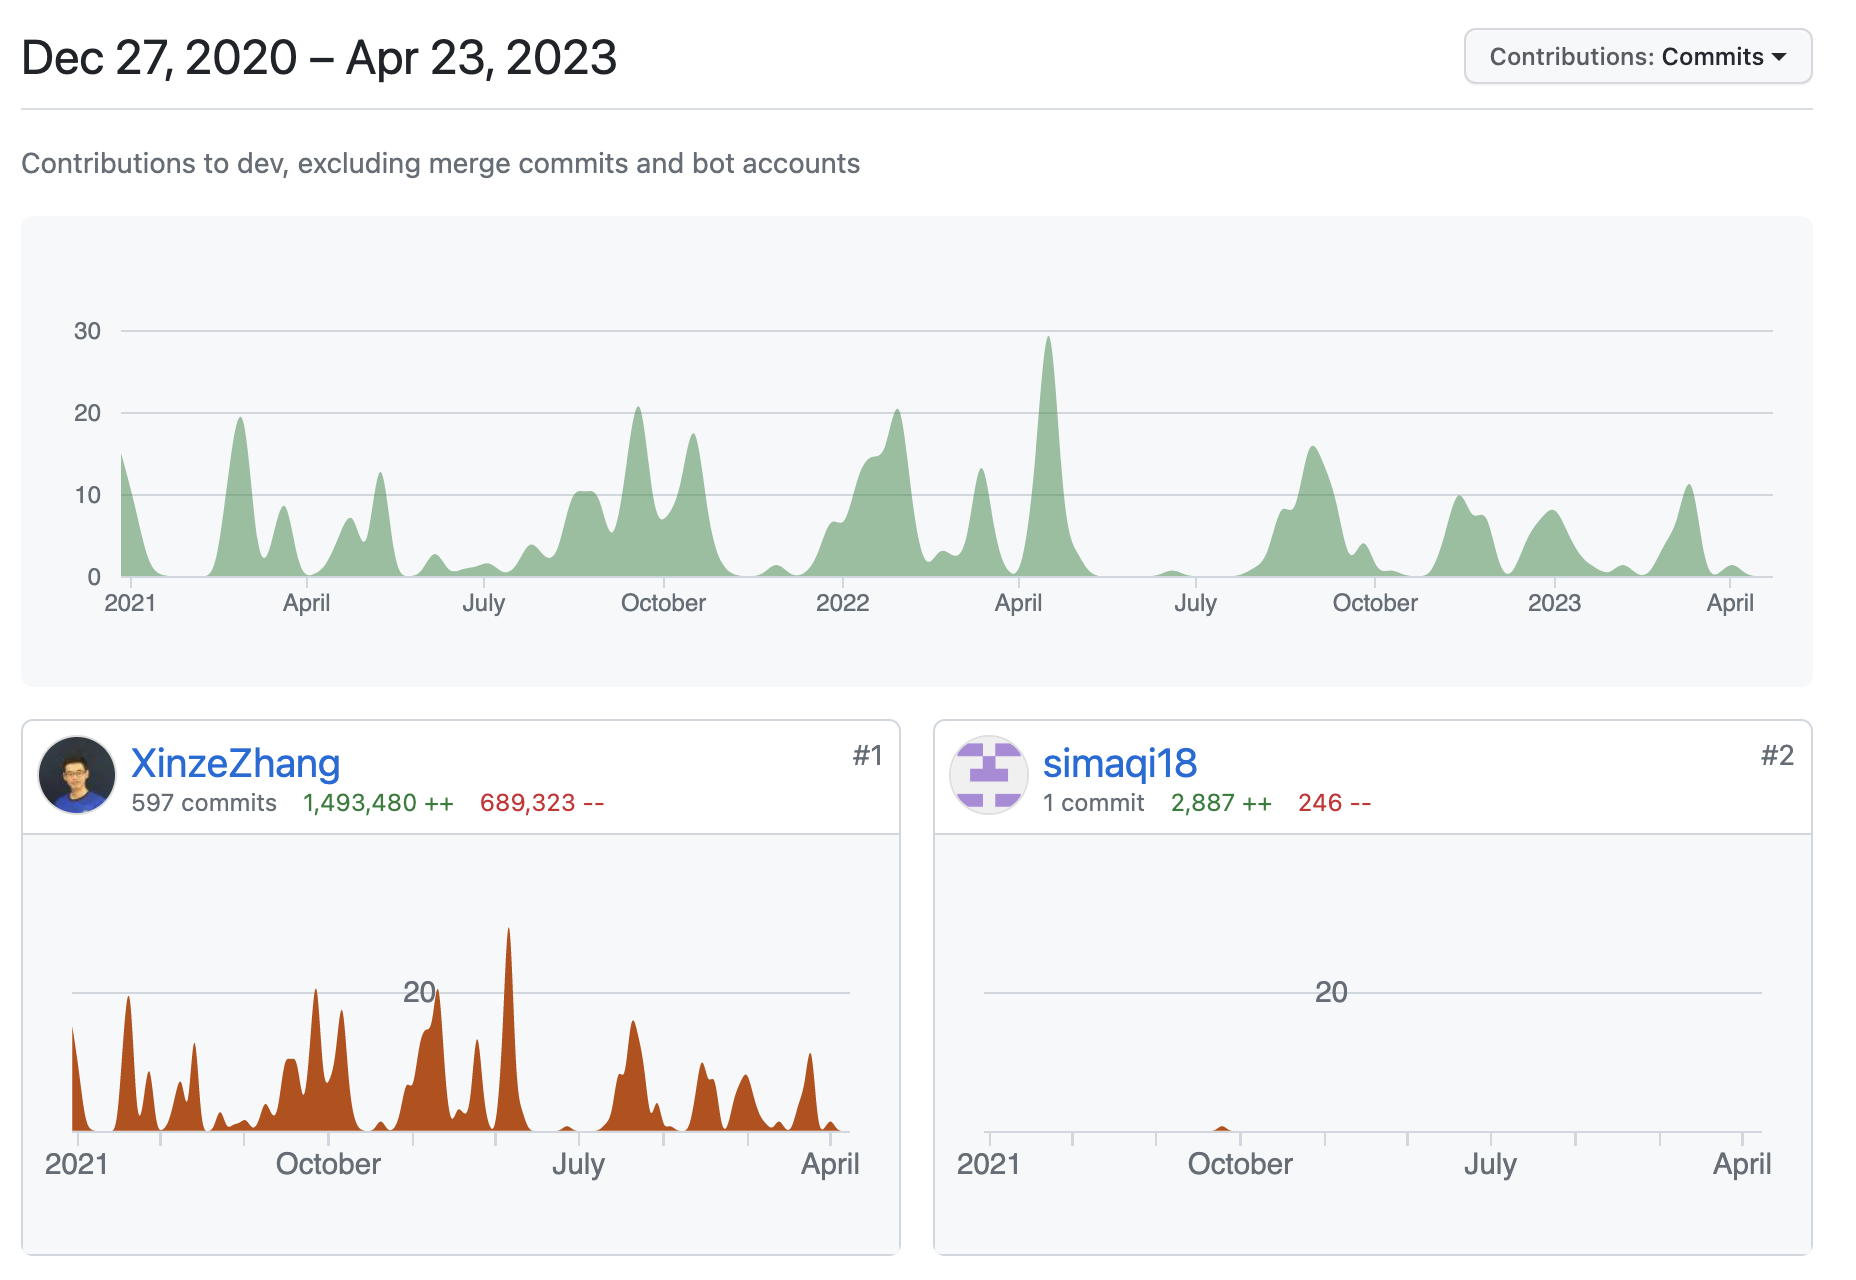
\includegraphics[width = 0.83\linewidth]{float/ch.univ/code2.png}

\end{frame}